% !TEX program = pdflatex
% !TEX options = -synctex=1 -interaction=nonstopmode -file-line-error "%DOC%"
% Group Theory Assignment 08
\documentclass[UTF8,10pt,a4paper]{article}
\usepackage[scheme=plain]{ctex}
\newcommand{\CourseName}{Group Theory}
\newcommand{\CourseCode}{PHYS2102}
\newcommand{\Semester}{Spring, 2020}
\newcommand{\ProjectName}{Assignment 08}
\newcommand{\DueTimeType}{Due Time}
\newcommand{\DueTime}{8:15, May 6, 2020 (Wednesday)}
\newcommand{\StudentName}{陈稼霖}
\newcommand{\StudentID}{45875852}
\usepackage[vmargin=1in,hmargin=.5in]{geometry}
\usepackage{fancyhdr}
\usepackage{lastpage}
\usepackage{calc}
\pagestyle{fancy}
\fancyhf{}
\fancyhead[L]{\CourseName}
\fancyhead[C]{\ProjectName}
\fancyhead[R]{\StudentName}
\fancyfoot[R]{\thepage\ / \pageref{LastPage}}
\setlength\headheight{12pt}
\fancypagestyle{FirstPageStyle}{
    \fancyhf{}
    \fancyhead[L]{\CourseName\\
        \CourseCode\\
        \Semester}
    \fancyhead[C]{{\Huge\bfseries\ProjectName}\\
        \DueTimeType\ : \DueTime}
    \fancyhead[R]{Name : \makebox[\widthof{\StudentID}][s]{\StudentName}\\
        Student ID\@ : \StudentID\\
        Score : \underline{\makebox[\widthof{\StudentID}]{}}}
    \fancyfoot[R]{\thepage\ / \pageref{LastPage}}
    \setlength\headheight{36pt}
}
\usepackage{amsmath,amssymb,amsthm,bm}
\allowdisplaybreaks[4]
\newtheoremstyle{Problem}
{}
{}
{}
{}
{\bfseries}
{.}
{ }
{\thmname{#1}\thmnumber{ #2}\thmnote{ (#3)} Score: \underline{\qquad\qquad}}
\theoremstyle{Problem}
\newtheorem{prob}{Problem}
\newtheoremstyle{Solution}
{}
{}
{}
{}
{\bfseries}
{:}
{ }
{\thmname{#1}}
\makeatletter
\def\@endtheorem{\qed\endtrivlist\@endpefalse}
\makeatother
\theoremstyle{Solution}
\newtheorem*{sol}{Solution}
\usepackage{graphicx}
\usepackage{subfigure}
\begin{document}
\thispagestyle{FirstPageStyle}
\begin{prob}
    Identify the point group that is obtained by combining the two symmetry elements in each case.
    \begin{enumerate}
        \item[(a)] A $2$-fold rotation axis and an inversion center.
        \item[(b)] Two mirror planes at right angles to each other.
        \item[(c)] A $2$-fold rotation axis and an intersecting mirror plane.
    \end{enumerate}
\end{prob}
\begin{sol}
    \begin{enumerate}
        \item[(a)] The $2$-fold rotation axis corresponds to rotation $C_2$. The inversion center corresponds to spatial inversion $I$. Combining $C_2$ and $I$, we get reflection in a horizontal plane $\sigma_h=C_2I=IC_2$, which is perpendicular to the $2$-fold rotation axis. Therefore, the point group is $C_{2h}=\{E,I,C_2,\sigma_h\}$.
        \item[(b)] The two mirror planes corresponds to two reflection operations $\sigma_v$ and $\sigma_d$, respectively. Since the two mirror planes are at right angles, combining $\sigma_v$ and $\sigma_d$, we get a $2$-fold rotation $C_2=\sigma_v\sigma_d=\sigma_d\sigma_v$, which is about the intersecting line of the two mirror planes. Therefore, the point group is $C_{2v}=\{E,C_2,\sigma_v,\sigma_d\}$.
        \item[(c)] The mirror plane must be perpendicular to the $2$-fold rotation plane, or the combination of the $2$-fold rotation and the reflection does not satisfy the associativity of the point group. The $2$-fold rotation axis corresponds to rotation $C_2$. The intersecting mirror plane corresponds to reflection $\sigma_h$. Combining $C_2$ and $\sigma_h$, we get a spatial reflection $I=C_2\sigma_h=\sigma_hC_2$. Therefore, the point group is $C_{2h}=\{E,I,C_2,\sigma_h\}$.
    \end{enumerate}
\end{sol}

\begin{prob}
    Let a rotation about an axis passing through the original and perpendicular to the $xOy$ plane through an angle of $\theta$ be represented by the matrix $R_{\theta}$ and a reflection in the line passing through the origin and making an angle of $\theta/2$ with the positive $x$ axis be represented by the matrix $S_{\theta}$. Show that $R_{\theta}$ and $S_{\theta}$ can be expressed as
    \[
        R_{\theta}=\left(\begin{matrix}
            \cos\theta&-\sin\theta\\
            \sin\theta&\cos\theta
        \end{matrix}\right),\quad S_{\theta}=\left(\begin{matrix}
            \cos\theta&\sin\theta\\
            \sin\theta&-\cos\theta
        \end{matrix}\right).
    \]
\end{prob}
\begin{sol}
    Let the coordinates of a fixed point $P$ before the operation be $r=\left(\begin{smallmatrix}
        x\\
        y
    \end{smallmatrix}\right)$, and the coordinates after be $r'=\left(\begin{smallmatrix}
        x'\\
        y'
    \end{smallmatrix}\right)$. If the operation is rotation about the axis passing through the original and perpendicular to the $xOy$ plane, the relations between the coordinates before and after the operation are (see figure \ref{2-R})
    \begin{align}
        x'=&x\cos\theta-y\sin\theta,\\
        y'=&x\sin\theta+y\cos\theta.
    \end{align}
    The above relations in the matrix form is
    \begin{align}
        r'=R_{\theta}r.
    \end{align}
    Therefore, the expression of $R_{\theta}$ is
    \begin{align}
        R_{\theta}=\left(\begin{matrix}
            \cos\theta&-\sin\theta\\
            \sin\theta&\cos\theta
        \end{matrix}\right).
    \end{align}
    If the operation is reflection in the line passing through the origin and making angle of $\theta/2$ with the positive $x$ axis, the relations between the coordinates before and after the operation are (see figure \ref{2-S})
    \begin{align}
        x'=&x\cos\theta+y\sin\theta,\\
        y'=&x\sin\theta-y\cos\theta.
    \end{align}
    The above relations in the matrix form is
    \begin{align}
        r'=S_{\theta}r.
    \end{align}
    Therefore, the expression of $S_{\theta}$ is
    \begin{align}
        S_{\theta}=\left(\begin{matrix}
            \cos\theta&\sin\theta\\
            \sin\theta&-\cos\theta
        \end{matrix}\right).
    \end{align}
    \begin{figure}[h]
        \centering
        \subfigure{
        \label{2-R}
        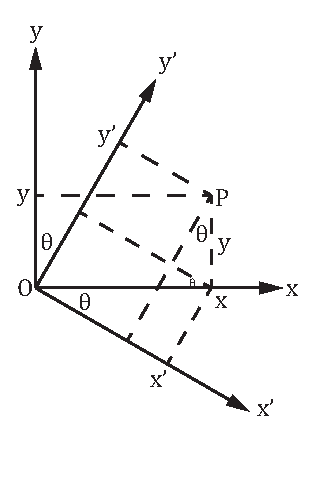
\includegraphics[width=.25\textwidth]{2-R.eps}}
        \subfigure{
        \label{2-S}
        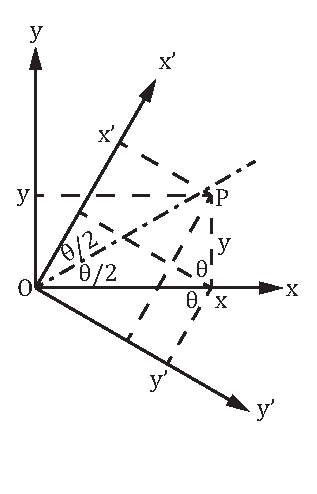
\includegraphics[width=.25\textwidth]{2-S.eps}}
        \caption{The scheme of two kinds of operations. Rotating of a point about an axis through an angle of $\theta$ is equivalent to rotating of the coordinate system about the same axis inversely through the angle of $\theta$. Reflecting of a point in a line is equivalent to reflecting of the coordinate system in the same line.}
    \end{figure}
\end{sol}

\begin{prob}
    Continue from the above problem.
    \begin{enumerate}
        \item[(a)] Compute the effect of rotating the vector $2e_x+3e_y$ conterclockwise about the origin through an angle of $\pi/2$ radians.
        \item[(b)] Compute the effect of reflecting the vector $e_x+e_y$ through the line $y=2x$.
        \item[(c)] Compute the effect of rotating the vector $e_y$ conterclockwise about the origin through an angle of $\pi/3$ radians and then reflecting through the line $y=2x$.
    \end{enumerate}
\end{prob}
\begin{sol}
    \begin{enumerate}
        \item[(a)] The coordinates after rotating the vector $2e_x+3e_y$ conterclockwise about the origin through an angle of $\pi/2$ radians is
        \begin{align}
            \left(\begin{matrix}
                x'\\
                y'
            \end{matrix}\right)=\left(\begin{matrix}
                \cos\frac{\pi}{2}&-\sin\frac{\pi}{2}\\
                \sin\frac{\pi}{2}&\cos\frac{\pi}{2}
            \end{matrix}\right)\left(\begin{matrix}
                2\\
                3
            \end{matrix}\right)=\left(\begin{matrix}
                -3\\
                2
            \end{matrix}\right).
        \end{align}
        Therefore, the effect of the rotation is to transform the vector $2e_x+3e_y$ into $-3e_x+2e_y$.
        \item[(b)] The line $y=2x$ make angle of $\theta/2=\arctan 2$ with the positive $x$ axis. The coordinates after reflecting the vector $e_x+e_y$ through this line is
        \begin{align}
            \left(\begin{matrix}
                x'\\
                y'
            \end{matrix}\right)=\left(\begin{matrix}
                \cos\theta&\sin\theta\\
                \sin\theta&-\cos\theta
            \end{matrix}\right)\left(\begin{matrix}
                x\\
                y
            \end{matrix}\right)=\left(\begin{matrix}
                -\frac{3}{5}&\frac{4}{5}\\
                \frac{4}{5}&\frac{3}{5}
            \end{matrix}\right)\left(\begin{matrix}
                1\\
                1
            \end{matrix}\right)=\frac{1}{5}\left(\begin{matrix}
                1\\
                7
            \end{matrix}\right).
        \end{align}
        Therefore, the effect of the reflecting is to transform the vector $e_x+e_y$ into $\frac{1}{5}e_x+\frac{7}{5}e_y$
        \item[(c)] The coordinates after rotating the vector $e_y$ conterclockwise about the origin through an angle of $\pi/3$ radians is
        \begin{align}
            \left(\begin{matrix}
                x'\\
                y'
            \end{matrix}\right)=\left(\begin{matrix}
                \cos\frac{\pi}{3}&-\sin\frac{\pi}{3}\\
                \sin\frac{\pi}{3}&\cos\frac{\pi}{3}
            \end{matrix}\right)\left(\begin{matrix}
                0\\
                1
            \end{matrix}\right)=\frac{1}{2}\left(\begin{matrix}
                -\sqrt{3}\\
                1
            \end{matrix}\right).
        \end{align}
        The coordinates after reflecting through the line $y=2x$ is
        \begin{align}
            \left(\begin{matrix}
                x''\\
                y''
            \end{matrix}\right)=\left(\begin{matrix}
                -\frac{3}{5}&\frac{4}{5}\\
                \frac{4}{5}&\frac{3}{5}
            \end{matrix}\right)\frac{1}{2}\left(\begin{matrix}
                -\sqrt{3}\\
                1
            \end{matrix}\right)=\frac{1}{5}\left(\begin{matrix}
                -3\sqrt{3}+4\\
                4\sqrt{3}+3
            \end{matrix}\right).
        \end{align}
        Therefore, the effect of the reflecting after the rotating is to transform the vector $e_y$ into $\frac{-3\sqrt{3}+4}{5}e_x+\frac{4\sqrt{3}+3}{5}e_y$.
    \end{enumerate}
\end{sol}

\begin{prob}
    Continue from the above problem.
    \begin{enumerate}
        \item[(a)] Show that $S_{\theta}S_{\psi}$ is a rotation and find the angle of rotation.
        \item[(b)] Show that $S_{\theta}S_{\psi}S_{\theta}=R_{-\psi}$.
        \item[(c)] Let $T_v$ be a translation through $v$, $T_vw=w+v$. Show that $T_{R_{\theta}v}R_{\theta}=R_{\theta}T_v$.
    \end{enumerate}
\end{prob}
\begin{sol}
    \begin{enumerate}
        \item[(a)] Since
        \begin{align}
            \nonumber S_{\theta}S_{\psi}=&\left(\begin{matrix}
                \cos\theta&\sin\theta\\
                \sin\theta&-\cos\theta
            \end{matrix}\right)\left(\begin{matrix}
                \cos\psi&\sin\psi\\
                \sin\psi&-\cos\psi
            \end{matrix}\right)=\left(\begin{matrix}
                \cos\theta\cos\psi+\sin\theta\sin\psi&\cos\theta\sin\psi-\sin\theta\cos\psi\\
                \sin\theta\cos\psi-\cos\theta\sin\psi&\sin\theta\sin\psi+\cos\theta\cos\psi
            \end{matrix}\right)\\
            \nonumber=&\left(\begin{matrix}
                \cos(\theta-\psi)&-\sin(\theta-\psi)\\
                \sin(\theta-\psi)&-\cos(\theta-\psi)
            \end{matrix}\right).
        \end{align}
        $S_{\theta}S_{\psi}$ is a rotation and the angle of the rotation is $\theta-\psi$ (counterclockwise).
        \item[(b)]
        \begin{align}
            \nonumber S_{\theta}R_{\psi}S_{\theta}=&\left(\begin{matrix}
                \cos\theta&\sin\theta\\
                \sin\theta&-\cos\theta
            \end{matrix}\right)\left(\begin{matrix}
                \cos\psi&-\sin\psi\\
                \sin\psi&\cos\psi
            \end{matrix}\right)\left(\begin{matrix}
                \cos\theta&\sin\theta\\
                \sin\theta&-\cos\theta
            \end{matrix}\right)\\
            \nonumber=&\left(\begin{matrix}
                \cos\theta\cos\psi+\sin\theta\sin\psi&-\cos\theta\sin\psi+\sin\theta\cos\psi\\
                \sin\theta\cos\psi-\cos\theta\sin\psi&-\sin\theta\sin\psi-\cos\theta\cos\psi
            \end{matrix}\right)\left(\begin{matrix}
                \cos\theta&\sin\theta\\
                \sin\theta&-\cos\theta
            \end{matrix}\right)\\
            \nonumber=&\left(\begin{matrix}
                \cos(\theta-\psi)&\sin(\theta-\psi)\\
                \sin(\theta-\psi)&-\cos(\theta-\psi)
            \end{matrix}\right)\left(\begin{matrix}
                \cos\theta&\sin\theta\\
                \sin\theta&-\cos\theta
            \end{matrix}\right)\\
            \nonumber=&\left(\begin{matrix}
                \cos(\theta-\psi)\cos\theta+\sin(\theta-\psi)\sin\theta&\cos(\theta-\psi)\sin\theta-\sin(\theta-\psi)\cos\theta\\
                \sin(\theta-\psi)\cos\theta-\cos(\theta-\psi)\sin\theta&\sin(\theta-\psi)\sin\theta+\cos(\theta-\psi)\cos\theta
            \end{matrix}\right)\\
            \nonumber=&\left(\begin{matrix}
                \cos(-\psi)&-\sin(-\psi)\\
                \sin(-\psi)&\cos(-\psi)
            \end{matrix}\right)=R_{-\psi}.
        \end{align}
        \item[(c)] Operating $T_{R_{\theta}v}R_{\theta}$ on an arbitrary vector $(x,y)^T$, we get
        \begin{align}
            \nonumber T_{R_{\theta}v}R_{\theta}\left(\begin{matrix}
                x\\
                y
            \end{matrix}\right)=&R_{\theta}\left(\begin{matrix}
                x\\
                y
            \end{matrix}\right)+R_{\theta}v=\left(\begin{matrix}
                \cos\theta&-\sin\theta\\
                \sin\theta&\cos\theta
            \end{matrix}\right)\left(\begin{matrix}
                x+v_x\\
                y+v_y
            \end{matrix}\right)\\
            \nonumber=&\left(\begin{matrix}
                (x+v_x)\cos\theta-(y+v_y)\sin\theta\\
                (x+v_x)\sin\theta+(y+v_y)\cos\theta
            \end{matrix}\right).
        \end{align}
        Operating $R_{\theta}T_v$ on $(x,y)^T$, we get
        \begin{align}
            R_{\theta}T_v\left(\begin{matrix}
                x\\
                y
            \end{matrix}\right)=R_{\theta}\left(\begin{matrix}
                x+v_x\\
                y+v_y
            \end{matrix}\right)=\left(\begin{matrix}
                (x+v_x)\cos\theta-(y+v_y)\sin\theta\\
                (x+v_x)\sin\theta+(y+v_y)\cos\theta
            \end{matrix}\right).
        \end{align}
        We find that
        \begin{align}
            T_{R_{\theta}v}R_{\theta}\left(\begin{matrix}
                x\\
                y
            \end{matrix}\right)=R_{\theta}T_v\left(\begin{matrix}
                x\\
                y
            \end{matrix}\right).
        \end{align}
        Due to the arbitrariness of $(x,y)^T$, $T_{R_{\theta}v}R_{\theta}=R_{\theta}T_v$.
    \end{enumerate}
\end{sol}

\begin{prob}
    Consider the point groups $C_{2v}$ and $D_{2h}$.
    \begin{enumerate}
        \item[(a)] Find all invariant subgroups of $C_{2v}$.
        \item[(b)] Find all invariant subgroups of $D_{2h}$.
    \end{enumerate}
\end{prob}
\begin{sol}
    \begin{enumerate}
        \item[(a)] The group $C_{2v}$ is
        \begin{align}
            C_{2v}=\{E,C_2,\sigma_v,\sigma_d\}.
        \end{align}
        The multiplication table of $C_{2v}$ is shown in table \ref{5-C2v-MT}.
        \begin{table}[]
            \centering
            \caption{The multiplication table of $C_{2v}$.}
            \label{5-C2v-MT}
            \begin{tabular}{c|cccc}
             & $E$ & $C_2$ & $\sigma_v$ & $\sigma_d$ \\ \hline
            $E$ & $E$ & $C_2$ & $\sigma_v$ & $\sigma_d$ \\
            $C_2$ & $C_2$ & $E$ & $\sigma_d$ & $\sigma_v$ \\
            $\sigma_v$ & $\sigma_v$ & $\sigma_d$ & $E$ & $C_2$ \\
            $\sigma_d$ & $\sigma_d$ & $\sigma_v$ & $C_2$ & $E$
            \end{tabular}
        \end{table}
        \\From the multiplication table, we get the subgroups of $C_{2v}$, as shown in table \ref{5-C2v-sg}.
        \begin{table}[h]
            \centering
            \caption{The subgroups of $C_{2v}$.}
            \label{5-C2v-sg}
            \begin{tabular}{ll}
            \hline
            Order & Subgroup(s) \\ \hline
            $s=1$ & $\{E\}$ \\
            $s=2$ & $\{E,C_2\},\{E,\sigma_v\},\{E,\sigma_d\}$ \\
            $s=4$ & $\{E,C_2,\sigma_v,\sigma_d\}$ \\ \hline
            \end{tabular}
        \end{table}
        \\From the multiplication table, we get the inverse of each element in $C_{2v}$ is itself:
        \[
            E^{-1}=E,\quad C_2^{-1}=C_2,\quad\sigma_v^{-1}=\sigma_v,\quad\sigma_d^{-1}=\sigma_d.
        \]
        For $X=E,C_2,\sigma_v,\sigma_d$,
        \begin{align}
            XC_2X^{-1}=E,
        \end{align}
        so the class of $C_{2v}$ constructed from $E$ is $\{E\}$.\\
        For $X=E,C_2,\sigma_v,\sigma_d$,
        \begin{align}
            XC_2X^{-1}=C_2,
        \end{align}
        so the class of $C_{2v}$ constructed from $C_2$ is $\{C_2\}$.\\
        For $X=E,C_2,\sigma_v,\sigma_d$,
        \begin{align}
            X\sigma_vX^{-1}=\sigma_v,
        \end{align}
        so the class of $C_{2v}$ constructed from $\sigma_v$ is $\{\sigma_v\}$.\\
        For $X=E,C_2,\sigma_v,\sigma_d$,
        \begin{align}
            X\sigma_dX^{-1}=\sigma_d,
        \end{align}
        so the class of $C_{2v}$ constructed from $\sigma_d$ is $\{\sigma_d\}$.\\
        The invariant subgroups of $C_{2v}$ are the subgroups consisting entirely of complete classes of $C_{2v}$:
        \[
            \{E\},\quad\{E,C_2\},\quad\{E,\sigma_v\},\quad\{E,\sigma_d\},\quad\{E,C_2,\sigma_v,\sigma_d\}.
        \]
        \item[(b)] The group $D_{2h}$ is
        \begin{align}
            D_{2h}=\{E,,I,C_2,C_2',C_2'',\sigma_h,\sigma_v,\sigma_v'\}.
        \end{align}
        The multiplication table of $D_{2h}$ is shown in table \ref{5-D2h-MT}.
        \begin{table}[h]
            \centering
            \caption{The multiplication table of $D_{2h}$}
            \label{5-D2h-MT}
            \begin{tabular}{c|cccccccc}
                & $E$ & $I$ & $C_2$ & $C_2'$ & $C_2''$ & $\sigma_h$ & $\sigma_v$ & $\sigma_v'$ \\ \hline
               $E$ & $E$ & $I$ & $C_2$ & $C_2'$ & $C_2''$ & $\sigma_h$ & $\sigma_v$ & $\sigma_v'$ \\
               $I$ & $I$ & $E$ & $\sigma_h$ & $\sigma_v'$ & $\sigma_v$ & $C_2$ & $C_2''$ & $C_2'$ \\
               $C_2$ & $C_2$ & $\sigma_h$ & $E$ & $C_2''$ & $C_2'$ & $I$ & $\sigma_v'$ & $\sigma_v$ \\
               $C_2'$ & $C_2'$ & $\sigma_v'$ & $C_2''$ & $E$ & $C_2$ & $\sigma_v$ & $\sigma_h$ & $I$ \\
               $C_2''$ & $C_2''$ & $\sigma_v$ & $C_2'$ & $C_2$ & $E$ & $\sigma_v'$ & $I$ & $\sigma_h$ \\
               $\sigma_h$ & $\sigma_h$ & $C_2$ & $I$ & $\sigma_v$ & $\sigma_v'$ & $E$ & $C_2'$ & $C_2''$ \\
               $\sigma_v$ & $\sigma_v$ & $C_2''$ & $\sigma_v'$ & $\sigma_h$ & $I$ & $C_2'$ & $E$ & $C_2$ \\
               $\sigma_v'$ & $\sigma_v'$ & $C_2'$ & $\sigma_v$ & $I$ & $\sigma_h$ & $C_2''$ & $C_2$ & $E$
            \end{tabular}
    \end{table}
    \\From the multiplication table, we get the subgroups of $C_{2v}$, as shown in table \ref{5-D2h-sg}.
    \begin{table}[h]
        \centering
        \caption{The subgroups of $D_{2h}$.}
        \label{5-D2h-sg}
        \begin{tabular}{ll}
            \hline
            Order & Subgroup(s) \\ \hline
            $s=1$ & $\{E\}$ \\
            $s=2$ & $\{E,I\},\{E,C_2\},\{E,C_2'\},\{E,C_2''\},\{E,\sigma_h\},\{E,\sigma_v\},\{E,\sigma_v'\}$ \\
            $s=4$ & $\{E,C_2,C_2',C_2''\},\{E,I,C_2,\sigma_h\},\{E,I,C_2',\sigma_v'\},\{E,I,C_2'',\sigma_v\},\{E,C_2,\sigma_v,\sigma_v'\}$ \\
            $s=8$ & $\{E,I,C_2,C_2',C_2'',\sigma_h,\sigma_v,\sigma_v'\}$ \\ \hline
        \end{tabular}
    \end{table}
    \\From the multiplication table, we get the inverse of each element in $C_{2v}$ is itself:
    \[
        E^{-1}=E,\quad I^{-1}=I,\quad C_2^{-1}=C_2,\quad(C_2')^{-1}=C_2',\quad(C_2'')^{-1}=C_2'',\quad\sigma_h^{-1}=\sigma_h,\quad\sigma_v^{-1}=\sigma_v,\quad(\sigma_v')^{-1}=\sigma_v.
    \]
    \end{enumerate}
    For $X=E,,I,C_2,C_2',C_2'',\sigma_h,\sigma_v,\sigma_v'$,
    \begin{align}
        XEX^{-1}=E,
    \end{align}
    so the class of $D_{2h}$ constructed from $E$ is $\{E\}$.\\
    For $X=E,,I,C_2,C_2',C_2'',\sigma_h,\sigma_v,\sigma_v'$,
    \begin{align}
        XIX^{-1}=E,
    \end{align}
    so the class of $D_{2h}$ constructed from $I$ is $\{I\}$.\\
    For $X=E,,I,C_2,C_2',C_2'',\sigma_h,\sigma_v,\sigma_v'$,
    \begin{align}
        XC_2X^{-1}=C_2,
    \end{align}
    so the class of $D_{2h}$ constructed from $C_2$ is $\{C_2\}$.\\
    For $X=E,,I,C_2,C_2',C_2'',\sigma_h,\sigma_v,\sigma_v'$,
    \begin{align}
        XC_2'X^{-1}=C_2',
    \end{align}
    so the class of $D_{2h}$ constructed from $E$ is $\{C_2'\}$.\\
    For $X=E,,I,C_2,C_2',C_2'',\sigma_h,\sigma_v,\sigma_v'$,
    \begin{align}
        XC_2''X^{-1}=C_2'',
    \end{align}
    so the class of $D_{2h}$ constructed from $C_2''$ is $\{C_2''\}$.\\
    For $X=E,,I,C_2,C_2',C_2'',\sigma_h,\sigma_v,\sigma_v'$,
    \begin{align}
        X\sigma_hX^{-1}=\sigma_h,
    \end{align}
    so the class of $D_{2h}$ constructed from $\sigma_h$ is $\{\sigma_h\}$.\\
    For $X=E,,I,C_2,C_2',C_2'',\sigma_h,\sigma_v,\sigma_v'$,
    \begin{align}
        X\sigma_vX^{-1}=\sigma_v,
    \end{align}
    so the class of $D_{2h}$ constructed from $\sigma_v$ is $\{\sigma_v\}$.\\
    For $X=E,,I,C_2,C_2',C_2'',\sigma_h,\sigma_v,\sigma_v'$,
    \begin{align}
        X\sigma_vX^{-1}=\sigma_v',
    \end{align}
    so the class of $D_{2h}$ constructed from $\sigma_v'$ is $\{\sigma_v'\}$.\\
    The invariant subgroups of $C_{2h}$ are the subgroups consisting entirely of complete classes of $C_{2v}$:
    \begin{gather*}
        \{E\},\{E,I\},\{E,C_2\},\{E,C_2'\},\{E,C_2''\},\{E,\sigma_h\},\{E,\sigma_v\},\{E,\sigma_v'\},\\
        \{E,C_2,C_2',C_2''\},\{E,I,C_2,\sigma_h\},\{E,I,C_2',\sigma_v'\},\{E,I,C_2'',\sigma_v\},\{E,C_2,\sigma_v,\sigma_v'\},\{E,I,C_2,C_2',C_2'',\sigma_h,\sigma_v,\sigma_v'\}
    \end{gather*}
\end{sol}
\end{document}